\subsection{Combinação de Imagens}
Combinação da imagem atual $A$ com uma segunda imagem $B$, com peso $\alpha$, resultando em $\alpha A + (1 - \alpha) B$. Tanto a imagem $B$ quanto o peso $\alpha$ devem ser passadao como argumentos, nessa ordem.

\begin{minted}{text}
    $ python main.py imagens/baboon.png combina imagens/butterfly.png 0.2
\end{minted}

\begin{listing}[H]
    \begin{minted}{python}
        def combinacao(A, B, alpha):
            img = A * alpha + B * (1 - alpha)
            return img.astype(np.uint8)
    \end{minted}

    \caption{Comando \texttt{combina IMAGEM ALPHA}}
\end{listing}

\begin{figure}[H]
    \centering
    \begin{subfigure}{0.45\textwidth}
        \centering
        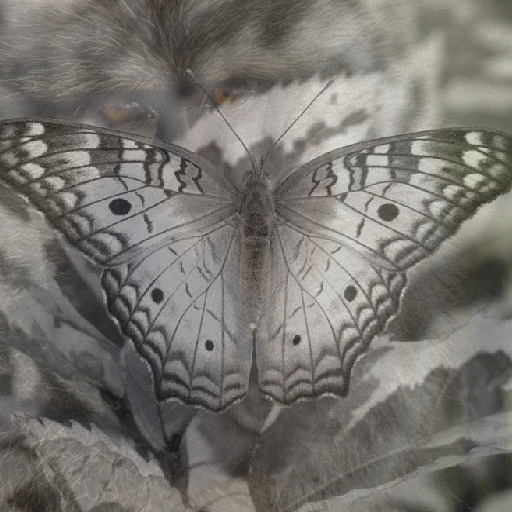
\includegraphics[width=6cm]{resultados/colormerg.png}
        \caption{\texttt{imagens/color.png}}
    \end{subfigure}%
    \begin{subfigure}{0.45\textwidth}
        \centering
        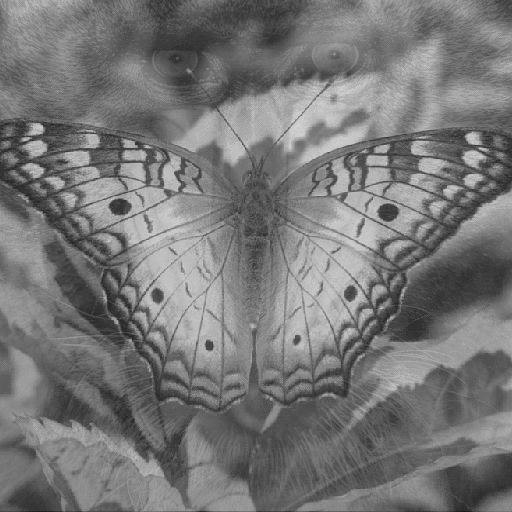
\includegraphics[width=6cm]{resultados/baboonmerg.png}
        \caption{\texttt{imagens/babooon.png}}
    \end{subfigure}

    \caption{Imagem combinada com \texttt{imagens/butterfly.png}, com $\alpha = 0.2$.}
\end{figure}

Usando a biblioteca OpenCV, essa função poderia ser implementada com o \pyline{addWeighted} \autocite{ref:addweighted}, como mostrada abaixo.

\begin{minted}{python}
    def combinacao(A, B, alpha):
        return cv2.addWeighted(A, alpha, B, 1-alpha, 0)
        # ou na arquitetura CUDA
        return cv2.cuda.addWeighted(A, alpha, B, 1-alpha, 0)
\end{minted}
